% Tik output from JumanG
\documentclass{article}
\usepackage{tikz}
\pagestyle{empty}
\usepackage{verbatim}
\begin{document}
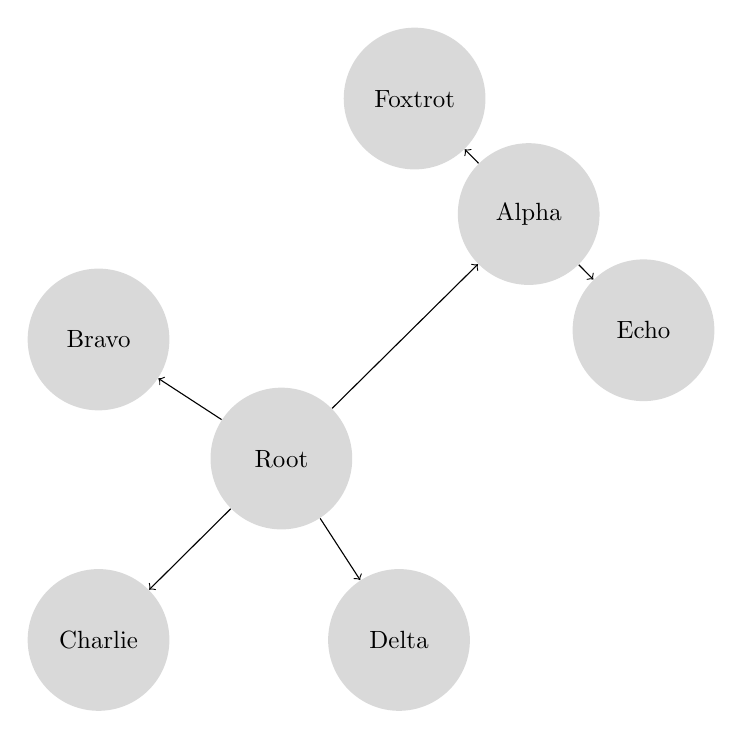
\begin{tikzpicture}[scale=.9, transform shape]
	\tikzstyle{every node} = [circle, fill=gray!30, minimum size = 2cm]
	\node (Charlie) at (-2.12, -2.12) {Charlie};
	\node (Delta) at (2.12, -2.12) {Delta};
	\node (Echo) at (5.57, 2.25) {Echo};
	\node (Bravo) at (-2.12, 2.12) {Bravo};
	\node (Alpha) at (3.95, 3.89) {Alpha};
	\node (Root) at (0.46, 0.44) {Root};
	\node (Foxtrot) at (2.34, 5.52) {Foxtrot};
	\draw [->] (Alpha)--(Echo);
	\draw [->] (Alpha)--(Foxtrot);
	\draw [->] (Root)--(Alpha);
	\draw [->] (Root)--(Bravo);
	\draw [->] (Root)--(Charlie);
	\draw [->] (Root)--(Delta);
\end{tikzpicture}
\end{document}
